\section{System Overview}
\label{sect:overview}
The kitting system that has been implemented as part of this work is a deliberative intelligent system based on the 4D/RCS 
reference model architecture \cite{Albus2000}. This architecture is a hierarchical architecture in which each echelon or level
follows a sense-model-act paradigm. The basic structure of the system may be seen in Figure \ref{fig:SenseModelAct}.
%
\subsection{Sense}
\label{subsection:Sense}
In order to sense action failures associated with kit building, it is necessary to be able to detect the six-degree of freedom pose of relevant objects in the
world. One issue with pose detection is the large number of potential target objects and object classes in the world. 
Both the number of objects and potential classes can be reduced by intelligently
selecting critical objects of interest that are tagged with predicted locations and object classes for the sensor system to track. This object selection, 
also known as focus of attention, is guided by
the Executor process with knowledge obtained from preconditions and effects of planned actions.
Actual algorithm development for pose and object detection is an active research area, and is beyond the scope of this article. 
For our purposes, 
we have assumed the use of a high-quality
system that is capable of recognizing a limited variety of items in a controlled environment and then determining each item's pose. 
%This is accomplished through simulation by using the Unified System for Automation and Robot Simulation (USARSim) \cite{Balakirsky2007}. As described in Section \ref{sect:future}, we intend to relax this assumption in the near future.
%
\begin{figure}[htb!]
\begin{center}
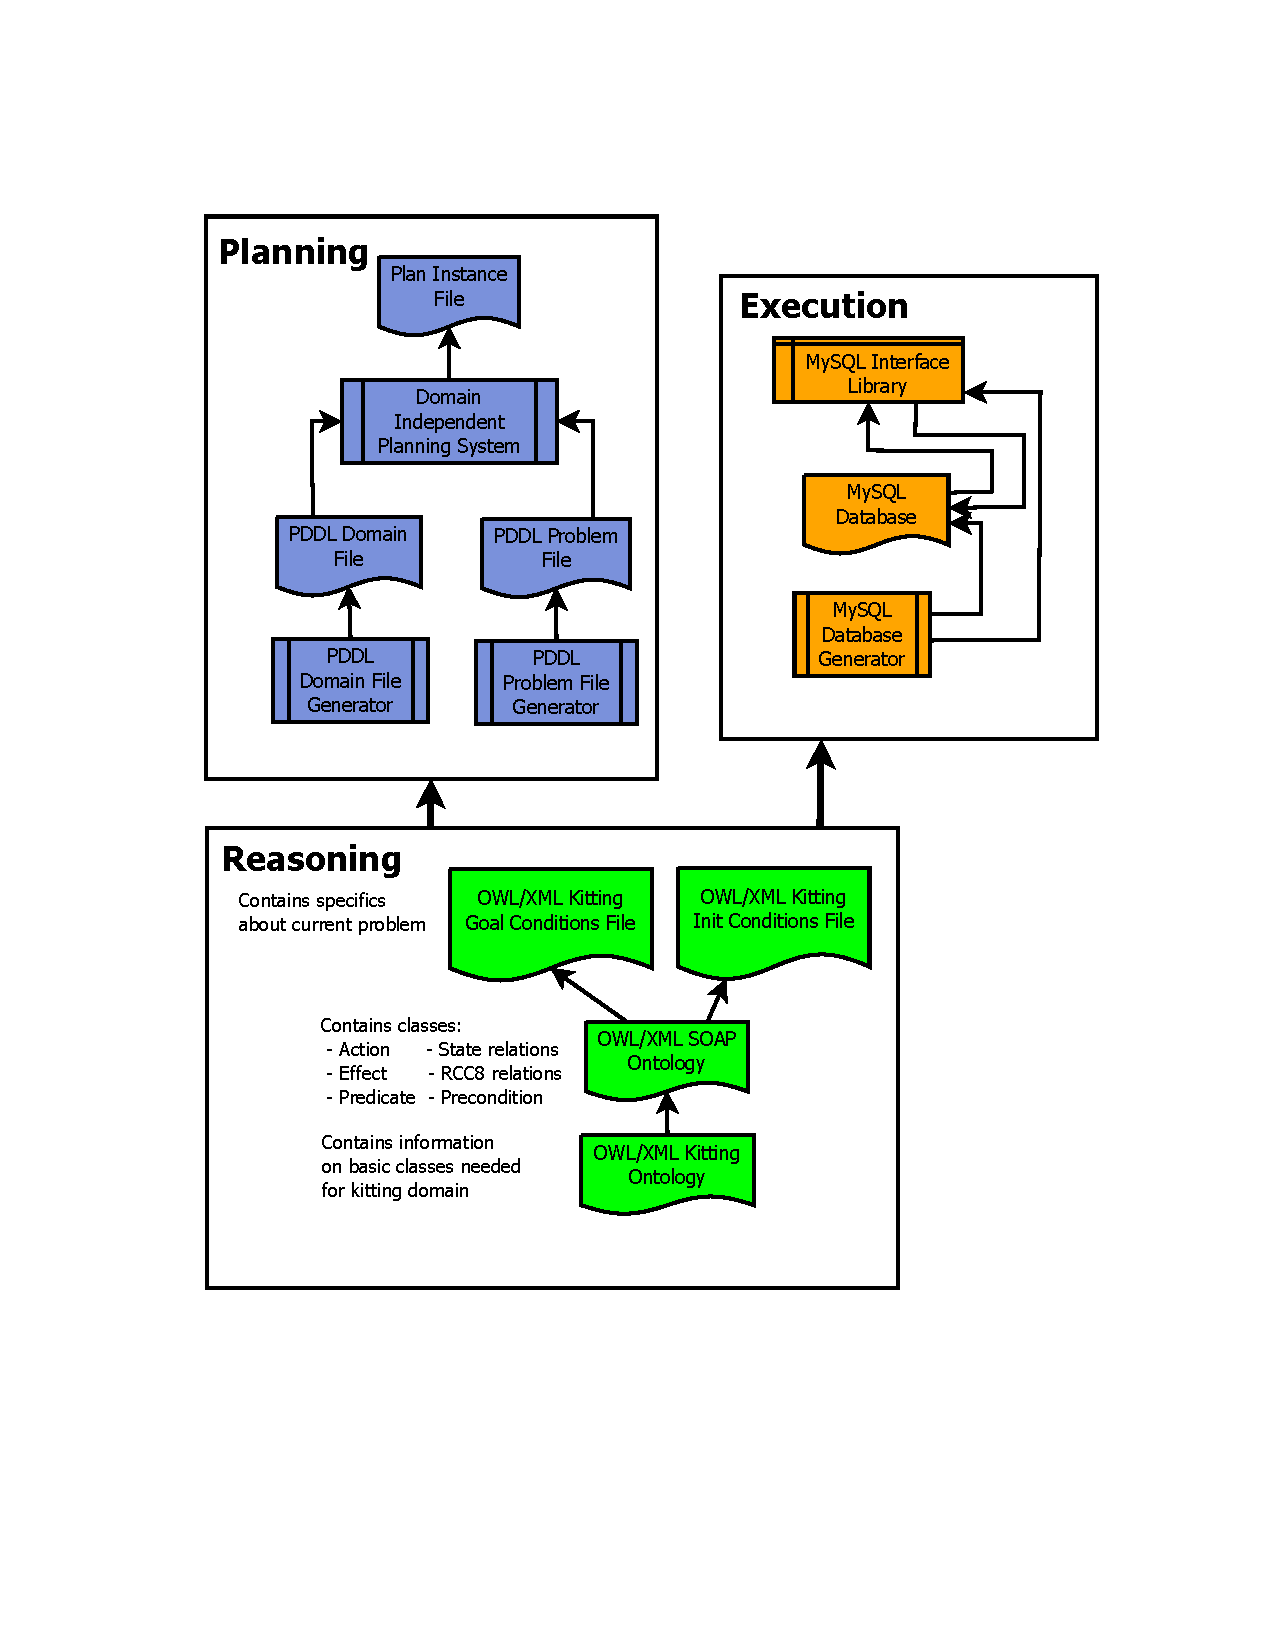
\includegraphics[width=8.5cm]{images/RITAWorldModel.pdf}
\caption{System World Model - The world model contains a Reasoning section that is based on an ontology shown in green,
a Planning section that is based on a Planning Domain Definition Language (PDDL) specification shown in blue, and an Execution section that is based on a dynamic database (MySQL) shown in orange.}
\label{fig:WorldModel}
\end{center}
\end{figure}
%
\subsection{Model}
\label{subsection:Model}
The world model that is being utilized is shown in Figure \ref{fig:WorldModel}. The model contains knowledge that is structured specifically for
reasoning, planning, and execution. All of the concepts necessary for the manufacturing domain under test are
encoded in the ontology that resides in the reasoning section of the model. The planning and execution sections of the model are automatically generated from
this section.
%
\subsubsection{Ontology --}
\label{sect:Ontology}
The reasoning portion of the world model is designed to contain all of the information needed to reason over and solve complex manufacturing
problems. The knowledge is represented in a Web Ontology Language (OWL) ontology that is structured in three parts. The first part of the ontology is an upper ontology
that contains generic information and classes that are needed for the domain of kit building. 
%
\begin{figure}[htb!]
\begin{center}
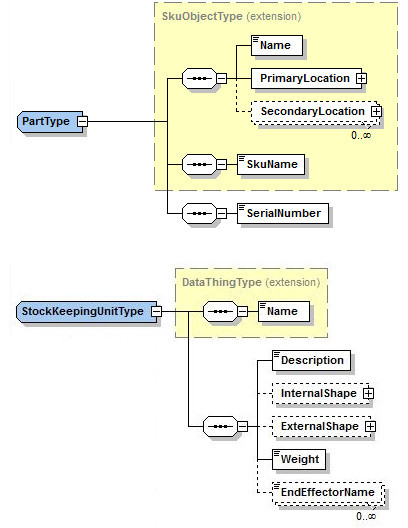
\includegraphics[width=8.5cm]{images/PartSKUV2.jpg}
\caption{Description of the PartType class that is designed to contain both static and dynamic information about particular parts and the StockKeepingUnitType class that contains static information about classes of parts.}
\label{fig:part}
\end{center}
\end{figure}
%
This area of the ontology contains information on basic elements such as a ``point" which is defined as a class that contains a name 
and a three-dimensional quantity, as well as complex types such as a ``part'', which is
shown in Figure \ref{fig:part}, and
contains elements such as the part's location and a name that references a stock keeping unit. The stock keeping unit contains static information on classes of parts such as the part's shape, weight, and the end effector that should be used for grasping the part. This information is utilized to create parameters for the Planning World
Model and the skeleton tables for the MySQL database of the Execution World Model.

Both static and dynamic information is represented in this
ontology and is automatically transitioned into the Planning and Execution areas of the world model. During system
operation,  dynamic information is updated in the Execution World Model.
More information on this portion of the ontology may be found in \cite{Balakirsky2012-1}.


The second part of the ontology (known as States, Ordering constraints, Actions, and Predicates or SOAP) contains the high-level concept of an action and all of the concepts 
that are required to support an action. In this case, a Planning Domain Definition Language (PDDL) \cite{PDDL} action is being represented, and this action is defined
 as an operator that causes one or more properties of an 
instance to change. Before this action may be
performed, certain preconditions must be satisfied, and after the action is performed, certain effects will take place. The action accepts parameters that specify the particular
instances that will be affected, where an instance refers to a physical object or piece of grounded data in the world. All of the necessary information for the automatic generation of the PDDL domain file required by the planning system is contained in this section of the ontology. The classes used to represent the actions in the ontology are provided in the
enumerated list shown below. 
\begin{enumerate}
\item \class{Action} -- An \class{Action} is the basic type that is used by a planning system to produce changes on the world. It has an \class{ActionPrecondition} that must be valid before the action may be executed and an \class{ActionEffect} that is expected to be produced by the action. Each action requires parameters that are used to specify which objects are being operated upon. These parameters are contained in the \class{ActionParameterList}. An \class{Action} has a unique name.
%
\item \class{ActionParameterList} -- Actions may have multiple parameters of different types that are represented by a class in the upper ontology. The \class{ActionParameterList} contains the particular action's parameters that are instances from the upper ontology. The order of the parameters in an  action also needs to be represented in the ontology. OWL has no built-in structure to represent an ordered list. In order to maintain parameter ordering, the parameter uses \emph{hasNextParameter} and \emph{hasPreviousParameter} to point to the next and the previous parameter in \class{ParameterList}, respectively.
%
\item \class{ActionPrecondition} -- An \class{ActionPrecondition} specifies necessary conditions that must be true in order for an action to be undertaken. It can consist of an \class{ActionPredicate}, an \class{ActionFunction}, an \class{ActionFunctionBool}, or a combination of these three classes. An \class{ActionPrecondition} belongs to one \class{Action}.
%
\item \class{ActionEffect} -- An \class{ActionEffect} specifies the results that are anticipated to occur as a result of a particular action. It can consist of an \class{ActionPredicate}, an \class{ActionFunction}, an \class{ActionFunctionBool}, or a combination of these three classes. An \class{ActionEffect} belongs to one \class{Action}. A negative \class{ActionPredicate} is represented with the declaration of \emph{hasEffect\_Predicate} within the OWL built-in property assertion \texttt{owl:NegativePropertyAssertion}.
%
\item \class{ActionPredicate} -- A predicate is used to specify a binary property of a single object, or a relationship between two objects. For example, the predicate \texttt{(robot-empty ?robot)} is true if the robot \texttt{?robot} is not holding anything. The predicate \texttt{(part-location-robot ?part ?robot)} is true only if the reference parameter \texttt{?part} is being held by the target parameter \texttt{?robot}.

An \class{ActionPredicate} represents these predicates. It has a unique name of type \texttt{string}, a reference parameter and a target parameter. The reference parameter is the first parameter in the predicate's parameter list and the target parameter is the second parameter in the predicate's parameter list. An \class{ActionPredicate} cannot have more than two parameters due to the inherent definition of predicates. In the case where an \class{ActionPredicate} has only one parameter, it is assigned to the reference parameter. 
%
\item \class{ActionFunction} -- In version 3 of the PDDL language, it is possible to use numeric functions that contain one or two parameters. For example, the function \texttt{(quantity-partstray ?partstray - PartsTray)} will return the number of parts that are contained in the parts tray \texttt{?partstray}, and the function
\texttt{(quantity-kit ?kit - Kit ?partstray - PartsTray)} will return the number of parts from parts tray \texttt{?partstray} that are currently in the kit \texttt{?kit}. The class \class{ActionFunction} is used to represent these functions. It has a unique name  of type \texttt{string} along with a reference parameter and a target parameter. The same rules apply to the definition and use of these two types of parameters as defined for \class{ActionPredicate}.
%
\item \class{ActionFunctionBool} -- In version 3 of the PDDL language, it is also possible to compare the results returned by two functions. The class \class{ActionFunctionBool} is used to represent these relationships. It has one or more subclasses that represent the type of relation (mathematical operator) between two \class{ActionFunction}s. Subclasses of \class{ActionFunctionBool} have a first \class{ActionFunction} that represents the \class{ActionFunction} on the left side of the operator and a second \class{ActionFunction} that represents the \class{ActionFunction} on the right side of the operator.
\end{enumerate}

The third part of the ontology contains specific instances needed for a particular kitting domain. For example, it will contain the definition of the finished kits that may be
constructed and specific information on the individual parts. One of the goals of this framework is to introduce additional agility into the kit building process. Therefore,
partial information is accepted and even encouraged for this area of the ontology. For the example of a part shown in Figure \ref{fig:part}, information on the SKU, grasp points 
(part of the ExternalShape or InternalShape), and name would be expected to be available at runtime. Information on the location of the part (PrimaryLocation) may not
become valid until after a sensor processing system has identified and located the particular part.
%
\subsubsection{Planning --}
The Planning Domain Definition Language (PDDL)  is an attempt by the domain independent planning community to formulate a standard language for planning. A community of planning researchers has been producing planning systems that comply with this formalism since the first International Planning Competition held in 1998. This competition series
continues today, with the seventh competition being held in 2011. PDDL is constantly adding extensions to the base language in order to represent more expressive problem domains. The representation in the world model is based on PDDL Version 3.

By placing the knowledge in a PDDL representation, the use of an entire family of open source planning systems such as the forward-chaining partial-order planning system from Coles et al. \cite{Coles.ICAPS.2010}
is enabled. In order to operate, the PDDL planners require a PDDL file-set that consists of two files that specify the domain and the problem.
From these files, the planning system creates an additional static plan file. Both the domain and problem file are able to be auto-generated from the ontology.

The generated static plan file contains a sequence of actions that will transition the system from the initial state to the goal state. In order to maintain flexibility, it is desired that detailed information that is subject to change should be ``late-bound'' to the plan. In other words, specific information is acquired directly before that information needs to be used by the system. This allows for last minute changes in this information. For example, the location of a kit tray on a work table may be different from run to run. However, one would like to be able to use the same planning sequence for constructing the kit independent of the tray's exact position.
To compensate for this lack of exact knowledge, the plans that are generated by the PDDL planning system contain only high-level actions.

As seen in Figure \ref{fig:WorldModel}, the planning world model framework contains generators that read the ontology and create
a standard PDDL domain and PDDL problem files. Any of the family of PDDL Version 3 compatible planning systems is then able to be
run on these files to create the static plan instance file. A representation of this plan may be stored in the ontology for future use.
%
\subsubsection{Execution --}
The execution world model is also built automatically from the ontology. This world model consists of a MySQL database and C\texttt{++} and Java
interfaces that provide for easy access to the data. The table skeletons are generated from the kitting ontology, and the tables are initially populated
with information from the initial and goal condition files. During plan execution, the Executor guides the sensor processing system
in updating the information in 
this section of the world model. All of the data structures encoded in the ontology are included in this representation. 
%An example 
%of the data tables that are created may be seen in Figure ?? for the Part class that is shown in Figure \ref{fig:part}. 
%
\subsection{Act}
\label{subsection:Act}
The actions that take place in the kitting work cell are coordinated by the Executor as illustrated in Figure \ref{fig:SenseModelAct}.  The Executor
reads PDDL actions as input and outputs a standardized set of low-level robot commands encoded in a language developed at the National Institute of Standards
and Technology (NIST) known as the  Canonical Robotic Command Language (CRCL) \cite{Balakirsky2012-1}. 

Before and after each high-level command
is executed, the Executor sends focus of attention information into the sensor processing system. This allows the sensor processing system to compute
the appropriate predicate relations that are required to verify the conditions necessary to carry out an action and that an action's execution has
been successful. Information on predicates is written to the world model by the sensing system and read from the world model by the Executor.
%
\\
\begin{algorithm}[h!]

 \KwData{ $kitToBuild$ }
 \KwResult{reports success or failure}
 	retrieve instance $PDDLInstance$ to construct kit $kitToBuild$\;
 	\For{each action $\textbf{A}$ in $PDDLInstance$}{
 		\For{each precondition $\textbf{P}$ of action $\textbf{A}$} {
			\If{$PredicateEvaluation(P)=false$}{
				report failure\;
			}
 		}
 		create set $S$ of Canonical Robot Control Language Commands\;
 		send set $S$ to Robot Controller for execution\;
 		\For{each effect $\textbf{E}$ of action $\textbf{A}$} {
			\If{$PredicateEvaluation(E)==false$}{
				report failure\;
			}
 		}
 		report action success\;
 	}
 	report plan success\;
\caption{{\sc BuildKit} -- Sequences the actions necessary to build a kit.}
\label{fig:buildkit}
\end{algorithm}
%